% ============================================================
% 机理图模板库（数学建模 · TikZ）
% 编译：xelatex mechanism-templates.tex   （中文必须 xelatex + ctex）
% 每个 tikzpicture 单独成页（standalone multi），可直接整段搬进自己的 .tex。
%
% 本机实测：PGF/TikZ 3.1.11a + MiKTeX，13 页 0 error / 0 overfull（2026-09-27）。
%
% 全部模板已按 references/tikz_rules.md 的两条铁律写：
%   铁律一：文字/数字/公式一律纯黑，彩色只给线条·曲线·箭头·点·区域填充
%   铁律二：带 fill= 的节点要设文字色必须写 text=black，绝不裸写 black
% 几何类配色 ≤3 色（黑 + gray!55 辅助 + 至多 1 个强调色）；框图类用方案 A（blue!80/blue!6 + teal!70）。
%
% 模板索引：
%   1  线性规划可行域图          2  相平面 / 向量场（零倾线+平衡点）
%   3  自由体受力图（隔离体）    4  光路系统图（满足透镜公式）
%   5  几何推导构造图（旗舰）    6  仓室传播链 SEIR
%   7  控制体微元示意            8  马尔可夫状态转移图
%   9  模型内部机理图（PINN）   10  指标层次结构图
%   11 元胞自动机邻域           12 临界位置双态对比
%   附 常用标注技巧片段（角度弧 / 双头尺寸 / 引线 / 装饰路径）
%
%    下面每个 tikzpicture 都刻意"只留图形元素 + 短符号标注"，一条说明文字都没焊进图里。
%    搬进论文时的正确嵌法（长公式推导一律写在图正下方的正文段落，不进图文件）：
%
%    \begin{figure}[H]\centering
%      \includegraphics[width=0.82\textwidth,keepaspectratio]{figures/mech_feasible_region.pdf}
%      \\[2pt]
%      \parbox{0.5\textwidth}{\footnotesize\centering
%        实线：约束边界\quad 虚线：等高线\quad ●：顶点\quad ●红：最优点}  % 只允许这种 ≤2 行窄图例
%      \caption{线性规划可行域与最优解的几何位置}\label{fig:mech-feasible}
%    \end{figure}
%
%    独立编译时（本文件这种 standalone）连这段图例都不该有——它会撑大 bounding box，
%    嵌进论文后主图被压扁、文字游离在图侧。
%
%    本文件踩过的坑（写新图时同样注意）：
%    grid[x step=..] 在 3.1.11a 报未知键，改用默认步长 `grid (X,Y)`
%    drop shadow 必须 \usetikzlibrary{shadows}
%    自定义样式名不要用 dash（与内置 /tikz/dash 冲突），改用 grpbox 之类
%    节点内文字不要出现裸 `/`（会被当 TikZ 路径分隔符）
%    分组虚线框必须在节点之前画，否则 fill=gray!2 会把下面的节点整片盖没
% ============================================================
\documentclass[multi=tikzpicture,border=3pt]{standalone}
\usepackage{ctex}
\usepackage{tikz}
\usetikzlibrary{arrows.meta,positioning,shapes.geometric,calc,patterns,
                decorations.pathmorphing,automata,quotes,shadows}

\begin{document}

% ============================================================
% 1 线性规划可行域图
% 题面自洽数据：max z=5x1+6x2, s.t. 2x1+3x2<=12, x1+x2<=5, x>=0
%   得可行域顶点 (0,0)(5,0)(3,2)(0,4)，最优解在两约束交点 (3,2)
% 技巧：可行域先 \fill 再画线（顺序即层级，免用 backgrounds）；等高线斜率 = -a/b
% 注意：最优点只写符号；约束方程用 sloped 骑在自身直线上，别另找地方塞
% ============================================================
\begin{tikzpicture}[scale=0.85]
  \draw[->] (0,0) -- (6.4,0) node[below left,font=\footnotesize] {$x_1$};
  \draw[->] (0,0) -- (0,5.4) node[below right,font=\footnotesize] {$x_2$};
  \fill[blue!10,fill opacity=0.45] (0,0) -- (5,0) -- (3,2) -- (0,4) -- cycle;
  \draw[blue!70!black,line width=0.9pt] (0,4) -- (6,0)
       node[pos=0.74,above,sloped,black,font=\scriptsize] {$2x_1+3x_2\le 12$};
  \draw[blue!70!black,line width=0.9pt] (0,5) -- (5,0)
       node[pos=0.34,above,sloped,black,font=\scriptsize] {$x_1+x_2\le 5$};
  % 目标函数等高线族（斜率 -5/6；最外一条正过最优点）
  \foreach \c in {2.5,3.5,4.5} \draw[gray!55,dashed] ({1.2*\c},0) -- (0,\c);
  % 优化方向：画在可行域外的空白处
  \draw[-{Stealth[length=3pt]},line width=0.9pt] (5.15,3.45) -- (5.75,4.17)
       node[above right,black,font=\footnotesize] {$\nabla z$};
  % 顶点（只给符号，不给解出的数值）
  \fill[black] (0,0) circle (1.5pt);  \node[black,font=\footnotesize,below left=1.5pt] at (0,0) {$O$};
  \fill[black] (5,0) circle (1.5pt);  \node[black,font=\footnotesize,below=2.5pt] at (5,0) {$A$};
  \fill[black] (0,4) circle (1.5pt);  \node[black,font=\footnotesize,left=2.5pt] at (0,4) {$D$};
  \fill[red!70!black] (3,2) circle (2.3pt);
  \draw[gray!60,thin] (3,2) -- ++(1.15,0.72)
       node[right,black,font=\footnotesize] {最优解 $B(x_1^*,x_2^*)$};
\end{tikzpicture}


% ============================================================
% 2 相平面 / 向量场
% 适用：微分方程稳定性、动力系统、捕食-竞争、SIR 定性相图
% 技巧：双 \foreach + \pgfmathsetmacro 画方向场；零倾线与坐标轴重合时把标签错开到轴端
% 注意：轨迹只画定性形状；数值解列表硬敲进 tex 属于数据图
% ============================================================
\begin{tikzpicture}[scale=0.95]
  \foreach \x in {-2,-1.4,-0.8,-0.2,0.4,1.0,1.6}{
    \foreach \y in {-1.6,-1.0,-0.4,0.2,0.8,1.4}{
      \pgfmathsetmacro{\vx}{-0.28*\y}
      \pgfmathsetmacro{\vy}{0.28*\x}
      \draw[gray!55,-{Stealth[length=1.8pt]}] (\x,\y) -- ++(\vx,\vy);
    }
  }
  \draw[->] (-2.4,0) -- (2.1,0) node[below left,black,font=\footnotesize] {$x$};
  \draw[->] (0,-1.9) -- (0,1.7) node[below left,black,font=\footnotesize] {$y$};
  \node[black,font=\scriptsize,anchor=west] at (1.32,0.42) {$\dot x=0$};
  \node[black,font=\scriptsize,anchor=west] at (0.12,1.32) {$\dot y=0$};
  % 代表性闭轨（中心型，定性示意）
  \draw[red!70!black,line width=1pt,dashed] (0,0) ellipse (1.25cm and 0.85cm);
  \draw[-{Stealth[length=3pt]},red!70!black,line width=1pt] (1.25,0) -- ++(-0.06,0.4);
  \fill[black] (0,0) circle (2pt);
  \draw[gray!60,thin] (0,0) -- (0.98,-0.98)
       node[right,black,font=\footnotesize] {平衡点 $(x_e,y_e)$};
\end{tikzpicture}


% ============================================================
% 3 自由体受力图（隔离体画法：不画支撑面，力不穿任何物体）
% 适用：力学/斜面/约束反力类赛题
% 技巧：力矢量彩色箭头从质心辐射；虚线只表示已撤去的约束方向；角度用 arc
% 注意：力符号 $mg$、$N$、$f$、$F$ 全是黑字，只有箭头有色
% ============================================================
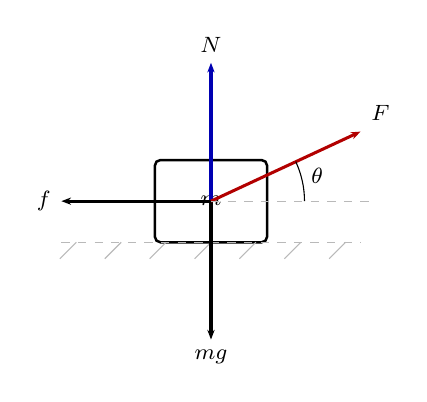
\begin{tikzpicture}[scale=0.95]
  \draw[black,line width=0.9pt,rounded corners=2pt,fill=white] (-0.75,-0.55) rectangle (0.75,0.55);
  \node[black,font=\footnotesize] at (0,0) {$m$};
  \coordinate (C) at (0,0);
  % 已撤去的支撑面（虚线 + 短剖面线）
  \draw[gray!55,dashed,thin] (-2.0,-0.55) -- (2.0,-0.55);
  \foreach \i in {-1.8,-1.2,-0.6,0,0.6,1.2,1.8}
    \draw[gray!55,thin] (\i,-0.55) -- ++(-0.22,-0.22);
  % 四个力
  \draw[black,-{Stealth[length=3.5pt]},line width=1.1pt] (C) -- (0,-1.85)
       node[below,black,font=\footnotesize] {$mg$};
  \draw[blue!70!black,-{Stealth[length=3.5pt]},line width=1.1pt] (C) -- (0,1.85)
       node[above,black,font=\footnotesize] {$N$};
  \draw[black,-{Stealth[length=3.5pt]},line width=1.1pt] (C) -- (-2.0,0)
       node[left,black,font=\footnotesize] {$f$};
  \draw[red!70!black,-{Stealth[length=3.5pt]},line width=1.1pt] (C) -- (2.0,0.93)
       node[above right,black,font=\footnotesize] {$F$};
  % 拉力与水平的夹角
  \draw[gray!55,dashed,thin] (C) -- (2.2,0);
  \draw[black] (1.25,0) arc (0:25:1.25);
  \node[black,font=\footnotesize] at (1.42,0.34) {$\theta$};
  %    正交分解的分量式写在正文，别在图上叠虚线（叠了容易和 mg 箭头混成一团）
\end{tikzpicture}


% ============================================================
% 4 光路系统图（几何严格自洽：f=1.5、u=3.0 得 v=3.0，像高 = -物高）
% 适用：透镜成像、反射折射、激光/集光类赛题
% 技巧：三条特殊光线必须共点于像点；尺寸线走图形外侧
% 注意：示意也要满足 1/u+1/v=1/f，画得不像物理上成立会被评委直接挑出来
% ============================================================
\begin{tikzpicture}[scale=0.9]
  \draw[gray!55,dashed] (-4.2,0) -- (4.2,0);
  \node[black,font=\scriptsize,anchor=west] at (3.55,-0.28) {主轴};
  \draw[blue!70!black,line width=1pt,fill=blue!8] (0,0) ellipse (0.19 and 1.5);
  \node[black,font=\footnotesize,anchor=south] at (0,1.56) {凸透镜};
  % 物
  \draw[black,-{Stealth[length=3pt]},line width=1pt] (-3,0) -- (-3,1.0)
       node[above,black,font=\footnotesize] {$AB$};
  % 三条特殊光线，全部会聚于像点 (3,-1)
  \draw[red!70!black,line width=0.8pt] (-3,1) -- (0,1);
  \draw[red!70!black,line width=0.8pt,-{Stealth[length=2.5pt]}] (0,1) -- (3,-1);
  \draw[red!70!black,line width=0.8pt] (-3,1) -- (0,0);
  \draw[red!70!black,line width=0.8pt,-{Stealth[length=2.5pt]}] (0,0) -- (3,-1);
  \draw[red!70!black,line width=0.8pt] (-3,1) -- (-1.5,0) -- (0,-1);
  \draw[red!70!black,line width=0.8pt,-{Stealth[length=2.5pt]}] (0,-1) -- (3,-1);
  % 焦点
  \foreach \p/\n in {(-1.5,0)/$F$,(-3,0)/$2F$,(1.5,0)/$F'$,(3,0)/$2F'$} {
    \fill[black] \p circle (1.5pt);
    \node[black,font=\footnotesize,above=2.5pt] at \p {\n};
  }
  % 像
  \draw[black,line width=0.9pt,dashed,-{Stealth[length=3pt]}] (3,0) -- (3,-1)
       node[below,black,font=\footnotesize] {$A'B'$};
  % 尺寸线
  \draw[<->,black,line width=0.7pt] (-3,-2.05) -- (0,-2.05)
       node[midway,above,black,font=\footnotesize] {$u$};
  \draw[<->,black,line width=0.7pt] (0,-2.05) -- (3,-2.05)
       node[midway,above,black,font=\footnotesize] {$v$};
\end{tikzpicture}


% ============================================================
% 5 几何推导构造图（本件旗舰模板）
% 题面自洽数据：观测点高 h=1.6 在 x=0.9；障碍高 H=1.15 在 x=2.6（低于视线）
%   临界视线 O 到 T 延长交地于 x*=6.94，盲区为 T-(2.6,0)-x* 三角形
% 技巧：主图只放"坐标系+已知量+辅助线+中间量符号"；标签挤同一焦点一律引线拉散；
%       局部放大另起 scope 画，且所有元素必须落在放大框内
% 注意：不许把三行公式说明焊进图内；图内的"数值"只能是题面给定常量
% ============================================================
\begin{tikzpicture}[scale=0.92]
  \draw[gray!50,very thin] (0,0) grid (7.2,3.6);
  \draw[->] (-0.3,0) -- (7.4,0) node[below left,black,font=\footnotesize] {$x$};
  \draw[->] (0,-0.3) -- (0,3.8) node[below left,black,font=\footnotesize] {$y$};
  \fill[pattern=north east lines,pattern color=gray!55] (0,-0.34) rectangle (7.4,0);
  \coordinate (O) at (0.9,1.6);
  \coordinate (T) at (2.6,1.15);
  \coordinate (P) at (6.94,0);
  % 盲区（先填区域，再画线，最后放文字）
  \fill[blue!12,fill opacity=0.45] (T) -- (P) -- (2.6,0) -- cycle;
  % 障碍
  \draw[blue!70!black,line width=1.3pt] (2.6,0) -- (T);
  % 临界视线（三点共线）
  \draw[red!70!black,line width=1pt,-{Stealth[length=3pt]}] (O) -- (T) -- (P);
  \fill[black] (O) circle (2pt);   \node[black,font=\footnotesize,left=2.5pt] at (O) {$O$};
  \fill[red!70!black] (T) circle (2pt);
  \fill[black] (P) circle (2pt);
  % 已知量
  \draw[<->,black,line width=0.7pt] (0.35,0) -- (0.35,1.6)
       node[midway,left,black,font=\footnotesize] {$h$};
  \draw[<->,black,line width=0.7pt] (2.98,0) -- (2.98,1.15)
       node[midway,right,black,font=\footnotesize] {$H$};
  \draw[<->,black,line width=0.7pt] (0.9,-0.75) -- (6.94,-0.75)
       node[midway,above,black,font=\footnotesize] {$d$};
  % 俯角 θ_c（视线在水平线下方，arc 取负角）
  \draw[black] ($(O)+(0.95,0)$) arc (0:-14.8:0.95);
  \node[black,font=\footnotesize] at (1.88,1.02) {$\theta_c$};
  % 焦点附近的标签用引线拉散
  \node[black,font=\footnotesize,anchor=south west] at (2.72,1.22) {临界顶点};
  \draw[gray!60,thin] (P) -- ++(0.5,0.62)
       node[right,black,font=\footnotesize] {遮蔽临界点 $x^{*}$};
  % 局部放大（元素全部落在框内）
  \begin{scope}[shift={(4.75,2.15)}]
    \draw[gray!45,dashed,rounded corners=2pt] (-0.12,-0.22) rectangle (2.42,1.28);
    \draw[blue!70!black,line width=1pt] (0.55,0) -- (0.55,0.72);
    \draw[red!70!black,line width=0.9pt] (0,0.95) -- (2.15,0.13);
    \fill[red!70!black] (0.55,0.72) circle (1.6pt);
    \node[black,font=\scriptsize,anchor=north east] at (2.3,1.2) {局部放大};
  \end{scope}
  \draw[gray!55,thin,-{Stealth[length=2pt]}] (3.05,1.62) -- (4.6,2.05);
\end{tikzpicture}


% ============================================================
% 6 仓室传播链（SEIR 类）
% 适用：传染病动力学、舆情扩散、物种迁移的机理示意
% 技巧：同类箭头用 bend 错开；速率标签用 above=<间距> 抬到框外，别压在框顶
% 注意：仓室名与速率符号都是黑字（只有箭头有色）；整句交代写正文
% ============================================================
\begin{tikzpicture}[
  font=\footnotesize,
  box/.style={draw=blue!80,fill=blue!6,line width=0.7pt,rounded corners=3pt,
              minimum width=1.0cm,minimum height=0.7cm,text=black,font=\bfseries,
              drop shadow={opacity=0.15,shadow xshift=0.5pt,shadow yshift=-0.5pt}},
  arw/.style={-{Stealth[length=3pt]},line width=0.8pt,color=blue!80},
  thin/.style={-{Stealth[length=2.5pt]},line width=0.6pt,color=gray!60}]
  \node[box] (S) at (0,0) {$S$};
  \node[box] (E) at (2.5,0) {$E$};
  \node[box] (I) at (5.0,0) {$I$};
  \node[box] (R) at (7.5,0) {$R$};
  \draw[arw] (S) -- (E) node[above=5pt,black,font=\scriptsize] {$\beta SI$};
  \draw[arw] (E) -- (I) node[above=5pt,black,font=\scriptsize] {$\sigma E$};
  \draw[arw] (I) -- (R) node[above=5pt,black,font=\scriptsize] {$\gamma I$};
  \draw[arw,bend right=20] (I.south) to node[below=6pt,black,font=\scriptsize]
       {隔离与治疗 $\delta I$} (R.south);
  \draw[thin] (S.west) -- ++(-0.7,0) node[left,black,font=\scriptsize] {$\Lambda$};
  \draw[thin] (S.south) -- ++(0,-0.5) node[left,black,font=\scriptsize] {$\mu$};
  \foreach \c in {E,I,R} \draw[thin] (\c.south) -- ++(0,-0.5);
  %    "各仓室均有自然死亡 μ"这类整句写进正文，不焊进图里
\end{tikzpicture}


% ============================================================
% 7 控制体微元示意
% 适用：热传导、扩散、渗流、流体等"取微元写守恒"的推导
% 技巧：微元淡填充 + 实线框；进/出通量箭头分置两侧，标签抬到箭头上方不压箭头
% ============================================================
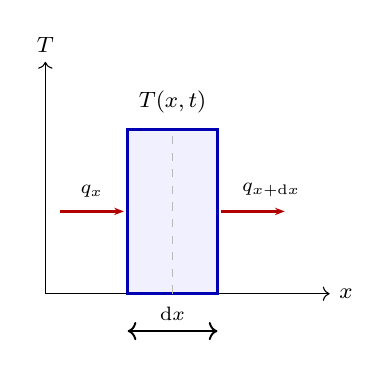
\begin{tikzpicture}[scale=0.95,font=\footnotesize]
  \draw[->] (0,0) -- (3.8,0) node[right,black] {$x$};
  \draw[->] (0,0) -- (0,3.1) node[above,black] {$T$};
  \draw[blue!70!black,line width=1pt,fill=blue!6] (1.1,0) rectangle (2.3,2.2);
  \draw[gray!55,dashed] (1.7,0) -- (1.7,2.2);
  \node[black,anchor=south] at (1.7,2.28) {$T(x,t)$};
  \draw[-{Stealth[length=3.5pt]},red!70!black,line width=1.1pt] (0.2,1.1) -- (1.05,1.1);
  \node[black,font=\scriptsize,anchor=south] at (0.62,1.16) {$q_x$};
  \draw[-{Stealth[length=3.5pt]},red!70!black,line width=1.1pt] (2.35,1.1) -- (3.2,1.1);
  \node[black,font=\scriptsize,anchor=south west] at (2.5,1.16) {$q_{x+\mathrm{d}x}$};
  \draw[<->,black,line width=0.7pt] (1.1,-0.5) -- (2.3,-0.5)
       node[midway,above,black,font=\scriptsize] {$\mathrm{d}x$};
  %    "截面积 A、密度 ρ、比热 c"这类参数罗列写进正文或图下 ≤2 行 parbox
\end{tikzpicture}


% ============================================================
% 8 马尔可夫状态转移图
% 适用：随机过程、队列/设备状态、天气与市场状态转移
% 技巧：automata 库；自环 loop above/below；对称转移用 bend 分两侧；边标签 quotes 语法
% 注意：转移概率只有题面给定的能写具体值，模型估出来的写 $p_{ij}$
% ============================================================
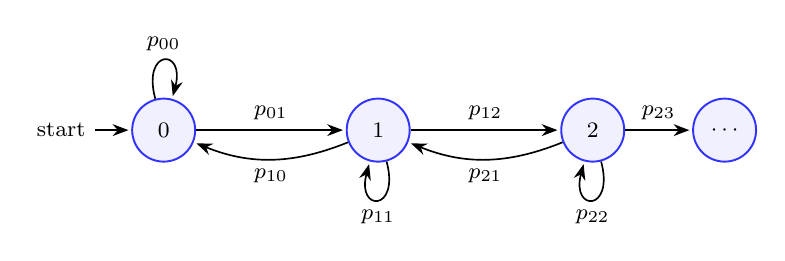
\begin{tikzpicture}[->,>=Stealth,shorten >=1pt,auto,node distance=1.9cm,semithick,
  font=\footnotesize,
  every state/.style={draw=blue!80,fill=blue!6,line width=0.7pt,text=black,minimum size=0.8cm}]
  \node[initial,state] (S0) {$0$};
  \node[state] (S1) [right=of S0] {$1$};
  \node[state] (S2) [right=of S1] {$2$};
  \node[state] (Sn) [right=0.85cm of S2] {$\cdots$};
  \path (S0) edge["$p_{01}$"] (S1)
        (S1) edge["$p_{12}$"] (S2)
        (S2) edge["$p_{23}$"] (Sn)
        (S1) edge[bend left=22,"$p_{10}$"] (S0)
        (S2) edge[bend left=22,"$p_{21}$"] (S1)
        (S0) edge[loop above,"$p_{00}$"] (S0)
        (S1) edge[loop below,"$p_{11}$"] (S1)
        (S2) edge[loop below,"$p_{22}$"] (S2);
\end{tikzpicture}


% ============================================================
% 9 模型内部机理图（PINN：物理约束建模的通用范式）
% 适用：PINN/算子学习/带物理约束的损失构成；也可套用到任意"多支路汇聚到一个损失"的模型
% 技巧：主链走水平直线；三条残差支路用"横向母线 + 垂直下探"分叉，天然不交叉；
%       反向传播回环走图的最外侧（左侧）用 dashed，绝不穿过主链节点
% 注意：换层数/参数量/超参是参数表的活，别堆进机理图
% 画 LSTM 三门同理：主记忆线走水平直线，三个门一律从正下方垂直进入 ×/+ 节点，
%   不要斜穿主链；候选支路从侧向弯入（to[bend left]）而不是从门下穿过
% ============================================================
\begin{tikzpicture}[
  font=\footnotesize,
  blk/.style={draw=blue!80,fill=blue!6,rounded corners=3pt,line width=0.7pt,text=black,
              minimum width=1.5cm,minimum height=0.72cm,
              drop shadow={opacity=0.15,shadow xshift=0.4pt,shadow yshift=-0.4pt}},
  sub/.style={draw=teal!70,fill=white,rounded corners=3pt,line width=0.6pt,text=black,
              minimum width=1.55cm,minimum height=0.62cm,font=\scriptsize},
  fl/.style={-{Stealth[length=2.8pt]},line width=0.8pt,color=blue!80},
  bk/.style={-{Stealth[length=2.8pt]},line width=0.7pt,color=gray!60,dashed}]
  \node[blk] (in) at (0,0) {$(x,t)$};
  \node[blk] (nn) at (2.9,0) {$\mathcal{N}_\theta$};
  \node[blk] (out) at (6.0,0) {$u_\theta(x,t)$};
  \draw[fl] (in) -- (nn);
  \draw[fl] (nn) -- (out);
  % 横向母线 + 三条垂直下探支路
  \draw[fl] (out.south) -- ++(0,-0.62) coordinate (bus);
  \draw[blue!80,line width=0.8pt] (3.6,-0.62) -- (8.4,-0.62);
  \node[sub] (r1) at (3.6,-1.75) {PDE 残差};
  \node[sub] (r2) at (6.0,-1.75) {初边值残差};
  \node[sub] (r3) at (8.4,-1.75) {数据拟合};
  \foreach \x/\n in {3.6/r1,6.0/r2,8.4/r3} \draw[fl] (\x,-0.62) -- (\n.north);
  \node[blk,minimum width=4.6cm] (loss) at (6.0,-3.2)
       {$\mathcal{L}=\mathcal{L}_{\mathrm{pde}}+\mathcal{L}_{\mathrm{bc}}+\mathcal{L}_{\mathrm{data}}$};
  \foreach \n in {r1,r2,r3} \draw[fl] (\n.south) -- (\n|-loss.north);
  \draw[bk] (loss.west) -- ++(-1.15,0) |- (nn.south)
       node[pos=0.72,left,black,font=\scriptsize] {反向传播};
\end{tikzpicture}


% ============================================================
% 10 指标层次结构图
% 适用：AHP / 熵权-TOPSIS / 模糊综合评价的指标体系示意
% 技巧：分组虚线框必须先画（否则 fill=gray!2 会把下面的节点整片盖没）；层名标签放框左上角外侧
% 注意：权重数值属求解结果，不进层次图
% ============================================================
\begin{tikzpicture}[
  font=\footnotesize,
  goal/.style={draw=blue!80,fill=blue!6,rounded corners=3pt,line width=0.7pt,text=black,
               minimum width=2.8cm,minimum height=0.7cm,
               drop shadow={opacity=0.15,shadow xshift=0.4pt,shadow yshift=-0.4pt}},
  crit/.style={draw=teal!70,fill=white,rounded corners=3pt,line width=0.6pt,text=black,
               minimum width=1.6cm,minimum height=0.6cm},
  idx/.style={draw=gray!50,fill=white,rounded corners=3pt,line width=0.5pt,text=black,
              minimum width=1.1cm,minimum height=0.5cm,font=\scriptsize},
  ln/.style={-{Stealth[length=2.2pt]},line width=0.5pt,color=black!70},
  grpbox/.style={draw=gray!40,dashed,fill=gray!2,rounded corners=4pt}]
  % 先画分组框
  \draw[grpbox] (-4.6,-2.62) rectangle (4.6,-1.78);
  \draw[grpbox] (-5.1,-4.82) rectangle (5.1,-3.98);
  \node[black,font=\scriptsize,anchor=south west] at (-4.6,-1.72) {准则层};
  \node[black,font=\scriptsize,anchor=south west] at (-5.1,-3.92) {指标层};
  % 再画节点
  \node[goal] (G) at (0,0) {目标层：综合评价 $A$};
  \node[crit] (B1) at (-3,-2.2) {准则 $B_1$};
  \node[crit] (B2) at (0,-2.2)  {准则 $B_2$};
  \node[crit] (B3) at (3,-2.2)  {准则 $B_3$};
  \node[idx] (C1) at (-3.9,-4.4) {$C_{1}$};
  \node[idx] (C2) at (-2.85,-4.4) {$C_{2}$};
  \node[idx] (C3) at (-0.6,-4.4) {$C_{3}$};
  \node[idx] (C4) at (0.6,-4.4) {$C_{4}$};
  \node[idx] (C5) at (2.85,-4.4) {$C_{5}$};
  \node[idx] (C6) at (3.9,-4.4) {$C_{6}$};
  \foreach \a/\b in {G/B1,G/B2,G/B3,B1/C1,B1/C2,B2/C3,B2/C4,B3/C5,B3/C6}
    \draw[ln] (\a.south) -- (\b.north);
  %    "权重 w_j 由求解给出、不入本图"这类交代写正文
\end{tikzpicture}


% ============================================================
% 11 元胞自动机邻域示意
% 适用：CA 演化、栅格扩散、空间传播、交通元胞模型
% 技巧：双层 \foreach 画栅格；邻域淡填充高亮；中心元胞用唯一强调色 + 黑体符号
% 注意：演化规则公式写进正文，不进图
% ============================================================
\begin{tikzpicture}[scale=0.55,font=\footnotesize]
  \foreach \i in {0,1,...,6} \foreach \j in {0,1,...,6}
    \draw[gray!45] (\i,\j) rectangle (\i+1,\j+1);
  \fill[blue!12] (2,2) rectangle (5,5);
  \foreach \p in {(2,2),(4,2),(2,4),(4,4)} \fill[gray!70] \p rectangle ++(1,1);
  \fill[red!70!black] (3,3) rectangle (4,4);
  \node[text=black,font=\bfseries] at (3.5,3.5) {$s_c$};
  \draw[<->,black,line width=0.8pt] (2,7.4) -- (5,7.4)
       node[midway,above,black] {Moore 邻域};
  \draw[gray!55,dashed] (2,7.28) -- (2,5.08);
  \draw[gray!55,dashed] (5,7.28) -- (5,5.08);
  %    演化规则 s_c^{t+1}=\mathcal{R}(\cdot) 写进正文
\end{tikzpicture}


% ============================================================
% 12 临界位置双态对比
% 适用：同一几何在"临界态 vs 一般态"下的差别（视角、覆盖、装满、相变）
% 技巧：实线=临界、虚线=一般；Δθ 的 arc 必须取在两条被比较的线之间，不是取在水平线上
% ============================================================
\begin{tikzpicture}[scale=0.9]
  \draw[->] (0,0) -- (4.9,0) node[below left,black,font=\footnotesize] {$x$};
  \draw[->] (0,0) -- (0,3.6) node[below left,black,font=\footnotesize] {$y$};
  \coordinate (P) at (0.8,0.8);
  \fill[black] (P) circle (1.8pt);
  \node[black,font=\footnotesize,anchor=north east] at (0.72,0.72) {$P$};
  \draw[red!70!black,line width=1.1pt] (P) -- (4.3,2.82);
  \node[black,font=\scriptsize,anchor=south west] at (3.6,2.9) {临界态};
  \draw[blue!70!black,line width=0.9pt,dashed] (P) -- (4.3,1.61);
  \draw[blue!70!black,line width=0.9pt,dashed] (P) -- (4.3,0.6);
  \node[black,font=\scriptsize,anchor=west] at (4.42,0.6) {一般态};
  % Δθ 夹在临界线与一般线之间：31.0° 到 12.9°
  \draw[black] ($(P)+(1.15*0.857,1.15*0.515)$) arc (31:12.9:1.15);
  \node[black,font=\footnotesize] at (2.1,1.32) {$\Delta\theta$};
\end{tikzpicture}


% ============================================================
% 附：常用标注技巧片段（单独成图，供拼进上面任意图）
% ============================================================
\begin{tikzpicture}[scale=0.95,font=\footnotesize]
  % (a) 角度弧：先移动再 arc，角度用符号不用数值
  \draw[black,line width=0.9pt] (0,0) -- (2.2,0) (0,0) -- (1.4,1.8);
  \draw[black] (0.7,0) arc (0:52:0.7);
  \node[black] at (1.0,0.3) {$\varphi$};
  % (b) 双头尺寸线：延伸线用细灰线，尺寸线走图形外侧（全部显式坐标，最稳）
  \draw[black,line width=0.9pt] (3.4,1.8) -- (5.0,1.8);
  \draw[gray!55,thin] (3.4,1.8) -- (3.4,1.0) (5.0,1.8) -- (5.0,1.0);
  \draw[<->,black,line width=0.7pt] (3.4,1.28) -- (5.0,1.28);
  \node[black] at (4.2,1.52) {$L$};
  % (c) 引线拉散：三个标签贴同一焦点时的唯一正解
  \coordinate (C) at (7.0,0.9);
  \fill[black] (C) circle (1.8pt);
  \draw[gray!60,thin] (C) -- ++(-0.6,0.72) node[above left,black,font=\scriptsize] {节点 $i$};
  \draw[gray!60,thin] (C) -- ++(0.6,-0.66) node[below right,black,font=\scriptsize] {节点 $i+1$};
  \node[black,font=\scriptsize,above=11pt of C] {弦长 $L_i$};
  % (d) 装饰路径：弹簧/波浪片段，嵌进力学或波动图
  \draw[black,line width=0.9pt,decorate,
        decoration={coil,aspect=0.5,amplitude=2.2mm,segment length=2.6mm}]
       (0,-1.5) -- (2.2,-1.5);
  \node[black,font=\scriptsize] at (1.1,-2.05) {弹簧 $k$};
  \draw[black,line width=0.9pt,decorate,decoration={snake,amplitude=1.3mm,segment length=4mm}]
       (3.2,-1.5) -- (5.6,-1.5);
  \node[black,font=\scriptsize] at (4.4,-2.05) {波动与扩散};
\end{tikzpicture}

\end{document}
